\documentclass[12pt,american,english, pointlessnumbers, abstracton, headsepline]{scrreprt}

\renewcommand{\familydefault}{\sfdefault}

%----------------------------------------------------------------------------------------------------------------------------------------------------------------------
% encoding
%----------------------------------------------------------------------------------------------------------------------------------------------------------------------
\usepackage[T1]{fontenc}
\usepackage[utf8]{inputenc}

\usepackage{geometry}

\geometry{verbose,tmargin=2.5cm,bmargin=2.5cm}
\pagestyle{plain}
\setlength{\parskip}{\medskipamount}
% \setlength{\parindent}{0pt}

\usepackage{color}
\usepackage{xcolor}
\usepackage[english]{babel}
\usepackage{array}
\usepackage{varioref}
\usepackage{textcomp}
\usepackage{multirow}
\usepackage{amsmath}
\usepackage{amsthm}
\usepackage{graphicx}
\usepackage{setspace}
\usepackage{nomencl}
\usepackage{tkz-graph}
\usepackage[hyphens]{url}
\usepackage{listings}
\usepackage{mdframed}
\usepackage{float}
\usepackage{alltt}
\usepackage[nounderscore]{syntax}
\usepackage{slashbox}

%----------------------------------------------------------------------------------------------------------------------------------------------------------------------
% nicer tables
%----------------------------------------------------------------------------------------------------------------------------------------------------------------------
\usepackage{booktabs}
\newcommand{\ra}[1]{\renewcommand{\arraystretch}{#1}}

%\usepackage[acronym]{glossaries}

%\newglossary{abbrev}{abs}{abo}{List of Abbreviations}
%
%\newglossaryentry{MS}{
%    name        = MS ,
%    description = mass spectroscopy ,
%    type        = abbrev
%}

%\makeglossaries

%----------------------------------------------------------------------------------------------------------------------------------------------------------------------
% syntax trees
%----------------------------------------------------------------------------------------------------------------------------------------------------------------------
\usepackage{qtree}

\setlength{\nomlabelwidth}{.20\hsize}
\renewcommand{\nomlabel}[1]{#1 \dotfill}

%\setlength{\nomitemsep}{-\parsep}

\makenomenclature

\setstretch{1.2}

\makeatletter

% Because html converters don't know tabularnewline
\providecommand{\tabularnewline}{\\}

% verschieden Symbole, Zeichen wie (c), �
\usepackage{textcomp,units}

%  more space between table and subtitle
\usepackage[tableposition=top]{caption}
\captionsetup[table]{skip=10pt}

%----------------------------------------------------------------------------------------------------------------------------------------------------------------------
% big chapter number indicator
%----------------------------------------------------------------------------------------------------------------------------------------------------------------------
\makeatletter
 \renewcommand*{\chapterformat}{% 
   \begingroup
     \setlength{\unitlength}{1mm}% 
     \begin{picture}(10,10)(0,5)
       \setlength{\fboxsep}{0pt}
       %\put(0,0){\framebox(20,40){}}% 
       %\put(0,20){\makebox(20,20){\rule{20\unitlength}{20\unitlength}}}% 
       \put(10,15){\line(1,0){\dimexpr 
           \textwidth-20\unitlength\relax\@gobble}}% 
       \put(0,0){\makebox(10,20)[r]{% 
           \fontsize{28\unitlength}{28\unitlength}\selectfont\thechapter 
           \kern-.05em% Ziffer in der Zeichenzelle nach rechts schieben 
         }}% 
       \put(10,15){\makebox(\dimexpr 
           \textwidth-20\unitlength\relax\@gobble,\ht\strutbox\@gobble)[l]{% 
             \ \normalsize\color{black}\chapapp~\thechapter\autodot 
           }}% 
     \end{picture} % <-- Leerzeichen ist hier beabsichtigt! 
   \endgroup 
}

\usepackage[automark]{scrpage2}
%\automark[chapter]{chapter}
\clearscrheadfoot
\ohead{\\\headmark}
\ihead{\includegraphics[scale=0.15]{logo.jpg}}%\pagemark}
\ofoot[\pagemark]{\pagemark}


% summary and abstract (english) on one page
\renewenvironment{abstract}{
    \@beginparpenalty\@lowpenalty
      \begin{center}
        \normalfont\sectfont\nobreak\abstractname
        \@endparpenalty\@M
      \end{center}
}{
    \par
}

%----------------------------------------------------------------------------------------------------------------------------------------------------------------------
% appearance optimization (commented out for faster compilation)
%----------------------------------------------------------------------------------------------------------------------------------------------------------------------
% optimization of appearance
\usepackage{microtype}
\usepackage{ %a4wide,
            ellipsis, fixltx2e, mparhack,
            booktabs, longtable
} 

\usepackage{ifpdf} % part of the hyperref bundle
\ifpdf
	%set fonts for nicer pdf view
	 \IfFileExists{lmodern.sty}{\usepackage{lmodern}}
	  {\usepackage[scaled=0.92]{helvet}
	    \usepackage{mathptmx}
	    \usepackage{courier} }
\fi

 % the pages of the TOC are numbered roman
 % and a pdf-bookmark for the TOC is added
 \pagenumbering{roman}
 \let\myTOC\tableofcontents
 \renewcommand\tableofcontents{
   %\pdfbookmark[1]{Contents}{}
   \myTOC
   \clearpage
   \pagenumbering{arabic}}

% cross refs as links
 \usepackage[colorlinks=true, bookmarks, bookmarksnumbered, bookmarksopen, bookmarksopenlevel=1,
  linkcolor=black, citecolor=black, urlcolor=blue, filecolor=blue,
  pdfpagelayout=OneColumn, pdfnewwindow=true,
  pdfstartview=XYZ, plainpages=false, pdfpagelabels,
  pdfauthor={LyX Team}, pdftex,
  pdftitle={LyX's Figure, Table, Floats, Notes, and Boxes manual},
  pdfsubject={LyX-documentation about figures, tables, floats, notes, and boxes},
  pdfkeywords={LyX, Tables, Figures, Floats, Boxes, Notes}]{hyperref}

% increased space between heading and table
\newcommand{\@ldtable}{}
\let\@ldtable\table
\renewcommand{\table}{ %
                 \setlength{\@tempdima}{\abovecaptionskip} %
                 \setlength{\abovecaptionskip}{\belowcaptionskip} %
                 \setlength{\belowcaptionskip}{\@tempdima} %
                 \@ldtable}

\renewcommand{\nomname}{Glossar}

\addto\captionsenglish{
  \renewcommand{\contentsname}
    {Table of Contents}
}

%----------------------------------------------------------------------------------------------------------------------------------------------------------------------
% colors
%----------------------------------------------------------------------------------------------------------------------------------------------------------------------
\definecolor{lightgray}{rgb}{0.8,0.8,0.8}

\definecolor{mygreen}{rgb}{0, 0.6, 0}
\definecolor{mygray}{rgb}{0.5, 0.5, 0.5}

\definecolor{numberbg}{rgb}{0.75, 0.75, 0.75}
\definecolor{numbercolor}{rgb}{0, 0, 0}
\definecolor{ballblue}{rgb}{0.13, 0.67, 0.8}

\AtBeginDocument{
  \def\labelitemiii{\(\circ\)}
}

\makeatother

\usepackage{listings}
\addto\captionsamerican{\renewcommand{\lstlistingname}{Listing}}
\addto\captionsenglish{\renewcommand{\lstlistingname}{Listing}}
\renewcommand{\lstlistingname}{Listing}

\makeindex

%----------------------------------------------------------------------------------------------------------------------------------------------------------------------
% quotations
%----------------------------------------------------------------------------------------------------------------------------------------------------------------------
\usepackage{epigraph}
\setlength\epigraphwidth{8cm}
\setlength\epigraphrule{0pt}

\usepackage{etoolbox}

%\makeatletter
%\patchcmd{\epigraph}{\@epitext{#1}}{\itshape\@epitext{#1}}{}{}
%\makeatother

\newcommand{
	\myquote
}[2]{
	\begin{mdframed}
		\vspace*{\fill}
		\epigraph{
			``#1''
		}{
			---#2
		}
	\end{mdframed}
}

%----------------------------------------------------------------------------------------------------------------------------------------------------------------------
% listings
%----------------------------------------------------------------------------------------------------------------------------------------------------------------------
\lstset{
	numbers=left,
	numbersep=8pt,
	numberstyle=\small\color{numbercolor},
	rulecolor=\color{numberbg},
	commentstyle=\color{mygreen},
	frame=single,
	framesep=0.5mm,
	framexleftmargin=15pt,
	fillcolor=\color{ballblue},
	tabsize=4,
	keywordstyle=\color{blue},
	morekeywords={*, SKIP, IF, THEN, ELSE, FI, WHILE, DO, OD},
	captionpos=b,
}

%definitions
\newtheorem{definition}{Definition}

\begin{document}

%----------------------------------------------------------------------------------------------------------------------------------------------------------------------
% table numbering
%----------------------------------------------------------------------------------------------------------------------------------------------------------------------
\renewcommand{\thetable}{T\arabic{table}}
\renewcommand{\thelstlisting}{L\arabic{lstlisting}}

%----------------------------------------------------------------------------------------------------------------------------------------------------------------------
% start
%----------------------------------------------------------------------------------------------------------------------------------------------------------------------
\titlepage
\begin{titlepage}

\begin{center}
\begin{tabular}{ccc}
 & \multirow{1}{*}{
\includegraphics{../bilder/logo_fb1}} & \tabularnewline
\end{tabular}
\par\end{center}

%\vspace{7cm}
\vfill

\begin{center}
\textbf{\Large{}Master Thesis}
\par\end{center}{\Large \par}

\begin{center}
{\large{}Design and implementation of a verifier for sequential programs
using the Hoare calculus}
\par\end{center}{\large \par}

\begin{flushleft}
{\Large{}\vfill
}
\par\end{flushleft}{\Large \par}

\begin{tabular}{ll}
submitted by:\hspace{1cm} & Florian Wege\tabularnewline
 & Student number: 15856\tabularnewline
 & Field of studies: Information and Communication Systems\tabularnewline
 & Merseburg University of Applied Sciences\tabularnewline
 & \tabularnewline
supervised by: & Prof. Dr. phil. Dr. rer. nat. habil. Michael Schenke\tabularnewline
 & Merseburg University of Applied Sciences\tabularnewline
 & Prof. Dr. rer. nat. habil. Eckhard Liebscher\tabularnewline
 & Merseburg University of Applied Sciences\tabularnewline
 & \tabularnewline
\multicolumn{2}{l}{Merseburg, \today}\tabularnewline
\end{tabular}

\end{titlepage}

\newpage{}

\tableofcontents{}

\newpage{}

\pagenumbering{roman}
\setcounter{page}{7}

\nomenclature{LAN}{Local Area Network}
% abbreviations:
%\newacronym{ny}{NY}{New York}

%\printglossary[type=abbrev]
\renewcommand{\nomname}{List of Abbreviations}
\printnomenclature

\newpage{}

\listoftables

\newpage{}

\listoffigures

\newpage{}

\pagenumbering{arabic}

\vspace{17.1mm}

\newpage{}

\chapter{Introduction}

\section{Motivation}
Since the introduction of computers, more and more of today's workings were shifted to digital processing. That transition streamlined a lot of things but also requested for a new profession facing up to controlling those machines, which would soon become known under the term software engineering. As there are a lot of processes to be described and accounted for, of course it would be bound to fan out and different engineers for different systems and hybrid forms would come to life. Programming has turned into a basic ability and some politicians actually want to integrate it into the curriculums of elementary schools.\footnote{\url{http://www.npr.org/sections/ed/2016/01/12/462698966/the-president-wants-every-student-to-learn-computer-science-how-would-that-work}} That discipline also experienced a certain trait of creativity. With the right idea in mind for an App, arranging the available components in a way of high usability, you can explore and look out for a market demand because a number of platforms and services are already in existence for you to unleash your ideas upon. Hardware, too, became more feasible and sophisticated in time but as the term discloses, software stands for a high level of malleability, which fosters trial-and-error-flavored development. When you develop for some platform, most of the details are abstracted, so, unless you are working with embedded systems, that require a close treatment, being aware of the inner workings at least partially has become increasingly unnecessary.

\myquote{At least once a semester I hear some kid yell, 'Wow! This is like magic!' and that really motivates them.}{Alfred Thompson, computer science teacher}

This is in contradistinction to the foundations of computer science, which seeks to formalize and systematically find solutions to problems. And in fact, as the application of software engineering progressed, the domain of topics enlarged. Questions of optimizations and concerns about security are slowly catching up and thus a greater insight is about to regain value.

Since it's more economic to do so, companies are content with the density of errors below a specified threshold. That is, the amount of errors per 1000 lines of code is measured and weighed against a target value fixed within the analysis phase. For applications where an error could cost the life of a human being, a limit of 0.5 (0.05\%) is the common pick. Though one may argue the risk should be reduced to zero and the worth of an individual is not up for quantification.

Besides most everyday business is already handled by software and there are a couple of different applications where utmost accuracy is key:

\begin{itemize}
	\item monetary transactions: automatic teller machines, to debit the right account, transfering ability where it's needed
	\item infrastructure: e.g. ensuring the proper behavior of vehicles
	\item dealing with customer (private) data
\end{itemize}

From a historical viewpoint, a number of different causes for misfunctioning software could be recorded: A comma in lieu of a dot, a wrong sign in front of a numeric expression, use of a wrong formula, racing conditions, an insufficient domain of definition, protocol errors, imprecision of floating point operations, overload, buffer overflow/underflow, non-considered cases and many more. Upcoming are trends like IoT (Internet of Things) or autonomous driving that pose new layers of networks and challenge established safety aspects. Another known concern is of economic nature: The later a software mistake is found, the more expensive it is to fix. After the development phase, the team that initially wrote the program often moved on to new tasks. Or in a case like the Mars rover, once deployed, you cannot just replace the software a posteriori. Moreover, often enough, the source code is not published, demands can change later on and glitches may manifest themselves without displaying symptoms at the beginning but which infect the system and which have an impact on the extendability. Thus it is vital to know that the software is indeed working correctly before its utilization.

\section{Analysis vs simulation}
To decrease the number of errors, a range of methods is at disposal. Most oftenly that involves peer reviews, i.e. an independent surveyor evaluates your code. Another idea is to simulate the behavior by carrying out dynamic test cases, directly running the code. Therefore, positive test cases are written that present well-formed inputs or conditions for an algorithm, then that algorithm is executed and the results are checked for integrity. Conversely, negative tests are to confirm bad input or precondition scenarios yield a proper error handling. The program is not supposed to end in an unregarded segmentation fault (stemming from an invalid access of memory), maybe should rather display a message box and append the information of the exception to a log file.

However, those tests cover but are part of the possible instances the code allows for, therefore fail to vindicate an overall correctness as a famous quote by E. W. Dijkstra alleges:

\myquote{Program testing can best show the presence of errors but never their absence.}{Edsger W. Dijkstra}

On the other hand, when speaking about verification in the environment of theoretical informatics, the term denotes an actual proof of the absence of errors within a program according to a specification using formal means. Hence it poses an exact method to evaluate the quality of a software, which, as hinted above, turns out to be crucial at some points, as a consequence rightfully enlarges the discipline of software engineering.

\section{Basic approaches}
Currently, there are two main approaches known to this stipulation: model checking and deductive means.

Model checking is the method of deciding whether a program or a model of it suffices a given specification by exploring its state-space.

A model is an abstraction of the reality. The idea is to examine the model in order to draw conclusions about the real system. It needs to be fitting to the task at hand, should be reduced as far as possible to simplify the issue but still contain all the relevant information. Different models can be mixed to acquire new information but such course of action is quick to decline the overall operability.

The state-space is a set or graph of constellations of the values of variables and the current point of execution. This vector describes the state of the program in its entirety. A verifier tool shifts between the states to find all possible execution paths. Those are then checked against conditions, e.g. invariants like a combination of variable values that should never occur. If an execution path should be found that violates these constraints, it will be returned and the programmer can observe the execution path that lead to the error to hopefully fix its cause. This approach basically traverses all possible variations before it marks the program as approved. That is why there is an exponential growth in computation time and required memory involved here, rendering the algorithm impractical fairly quickly. Model checking also necessitates a closed, finite system (or an algorithm to render it as such). Otherwise you could keep allocating memory and the number of states would not exhaust, thus the verifier may never come to a conclusion. Dynamic data structures may be examined by specialized methods like shape analysis\footnote{\url{https://en.wikipedia.org/wiki/Shape_analysis_(program_analysis)}}.

Both the model and the specifications are described in dedicated languages that allow the verifier to work with. Due to the intent of exploring the state space, the modeling language must project a finite state machine. Examples are PROMELA (Process Meta Language), Timed Automata or Petri nets. The specifications or properties checked for are usually decorated by logical expressions like temporal logic as introduced in programs by A. Pnueli\footnote{\url{http://fi.ort.edu.uy/innovaportal/file/20124/1/49-pnueli_temporal_logic_of_programs.pdf}}, are tacit (a division by zero should never occur) or may be integrated in the modeling language itself, e.g. PROMELA permits to insert assertions as part of the control flow.\footnote{\url{https://en.wikipedia.org/wiki/Model_checking}}

%In the Java programming language, more specifically the runtime environment, there is a verifier checking the used classes for specific illegal structure, including:
%
%\begin{itemize}
%	\item Usage of uninitialized variables
%	\item Violation of access rights (e.g. write to a private variable from another scope)
%\end{itemize}
%
%\footnote{\url{http://www.informit.com/articles/article.aspx?p=1187967&seqNum=2}}

Another axiomatic way of verifying a program and the method presented to be in this paper is resolution of theorems. This idea was first introduced by Alan Turing on a conference in 1949. Due to typographical mistakes and other circumstances, it went hidden for a bit but later on other researches would have retaken the topic. But the important thing was to notice that the problem could be modularized and that a program (Turing used flowcharts back then) could be decorated with assertions. In 1969, Tony Hoare invented a set of axioms and rules, so-called Hoare triples, that would point out a relation between an elementary program instruction or control flow and its effect on what can be logically assumed from what the semantics of this piece of code are to induce. For example the following listing increments a numerical variable 'x' by 1.

\begin{lstlisting}[caption={First listing}]
	x=x+1
\end{lstlisting}

Now it can be said that prior to this assignment, the variable was lower by 1 compared to afterwards. Or more generally, before the assignment, every occurence of 'x' had been substituted by the expression of the new value.

\begin{figure}
	\begin{lstlisting}[caption={Disadvantages of state-space exploration}]
		PRE{}
			z=x+y;
			z=z*2;
			z=z-(x+y)
		POST{z==x+y}
	\end{lstlisting}
\end{figure}

The above code snippet shall serve as an easily visible example for when deductive means outclass the procedure of state exploration. Assuming that x and y are only 2 byte integer variables and may take any value in their data type domain, that totals the combination of 32 bits or over 4 billion possibilities to check the post condition for, which is what state exploration would do. On the other hand, a human being should be able to recognize the pattern easily. By substitution, one could argue the assignments could be reduced to a single one (z=x+y) and that straight seems to match the post condition. So does the above program fulfill the surrounding specification? Maybe, maybe not. It should be considered that, first off, the conditions between the curly braces possess their own language with their own semantics, e.g. the operators may have their own meaning. Secondly, those are not exactly mathematical expressions. As hinted by x and y being 2 byte integer variables, z too might be restricted, thus the add and multiplication instructions may cause a buffer overflow, whereupon the semantics would have been altered by the substitution then. So of course it depends on the underlying system and that system respectively the semantics of the language have to be well-known in detail. Other than that, an axiomatic theorem solver like the human would identify the pattern, apply rules on the structure of the program to see what can be derived from it and then make statements about it.

However, deductive program verification comes with its own set of problems: Those usually revolve around the elementary control flow constructs of imperative programming languages and the implications of those are not necessarily assessable in their entirety. The question whether a predicate logic expression implicites another is known to be undecidable in general. Furthermore, the calculus viewed here only establishes relationships.

From theoretical informatics it can be stated that, in general, it is impossible to say if a program satisfies a set of specifications of any kind. However, it becomes more feasible when narrowed down to classes of programs and regarded languages.

\section{What the paper is about}
The objective of this paper shall be to outline the Hoare calculus, make a design for a verifier that would present how it is applied starting from a raw string input, how the mathematical formulae that come with it could be transcribed to imperative algorithms and at which points the interaction with a human user is still required. The elaborated design is then to be implemented in Java along with an appropriate graphical user interface to portray the procedure.

To conclude the introduction, it should be stated that both model checking and theorem solving rely on a proper specification of the issue. If that is already wrong, which may be the case, since the specification needs a strict formalization as well, a verification will not help because it does not know the client's intentions.

Figure \ref{figure:taskToProgram} reveals more origins of error. Even when establishing specifications and a model and even obtaining the program by transformation of the model in the target language, there are still risks of human failings in between that may falsify the verification result (and the tooling must be assumed to be working flawlessly). That poses another reason why even a formal verification should only be seen as an additional scheme in the quality assurance environment.

\begin{figure}
	\label{taskToProgram}
	\caption{From definition of task to program}
\end{figure}

language extension by assertions/annotations
raw string -> tokens -> syntax tree -> deduction

%\section{On correctness of programs}
%
%What declares a program as correct? For sure, the answer to this question is as vague as it gets: if it fulfills the specifications. There are a number of pretty straightforward desires that are common ones: the program should terminate, no runtime errors are to occur. If we include parallel programs, some more bad stuff can happen like deadlocks or livelocks.
%
%\begin{tikzpicture}
%	\GraphInit[vstyle = Shade]
%	%\tikzset{LabelStyle/.style = {rectangle, rounded corners, draw, minimum width = 2em, fill = yellow!50, text = red, font = \bfseries}}
%	\tikzset{VertexStyle/.append style = {inner sep=2pt, font=\Large\bfseries}}
%	\tikzset{EdgeStyle/.append style = {->, bend left}}
%	\SetGraphUnit{5}
%	\Vertex{Specification}
%	\WE(Specification){Client}
%	\EA(Specification){Model}
%	\Edge[label=still unsafe](Client)(Specification)
%	\Edge[label=to be verified](Model)(Specification)
%\end{tikzpicture}

\chapter{Preliminaries}

\section{Overview}

Before plunging into the core topic of this paper, it appears necessary to formalize the target of a prospective verifier. In order to make statements about the validity of a program, whether it holds to certain properties or not, both the program and the properties should be fixated. What could be considered secure knowledge anyway? Such a holistic view only makes sense under the presumption that some basic ideas can already be regarded as irrevocably intrinsic and then means of induction, analogy etc. are used to widen the scope and to declare more statements as compatible to the existing knowledge base, verifying them or, if they appear as contradictory, one will have to object them.

And the strategy here is likewise: To know if a program fulfills some conditions, the meaning of the program and the conditions has to be precise. Since this entails lots and lots of programs and conditions in general, it becomes evident that rather than manually and pointlessly contemplating all possible variations, it deems better to ascribe it to some underlying scheme that can be unfolded on demand. Therefore the meaning, also called the semantics, of a program (and later also those of conditions) is inductively synthesized using a model kit relating to a set of basic entities. Prior to determining the semantics, these entities also have to be identified as such, which is the part of the syntax analysis and shall be depicted as well.

Therefore the schedule is as follows: The rest of this chapter will give some further classification, tease about the purport and hand over a short preview. It may be skipped if the reader is fond of the contextual knowledge. Chapter ~\ref{ch:Introduction of language} will formally start with the definition of a language, how are they characterized and how are they processed. Then the specific language subject to this paper and whose programs are to be verified is firmly presented along with some simple remarks about its significance. Afterwards, in the dedicated ~\ref{ch:Semantics} chapter, these semantics are going to be formalized and, moreover, the type of semantics and how to continue with it are explained. The ~\ref{ch:How to prove} chapter reasons about using the obtained semantics, talks about the notion of correctness and introduces assertions by extending the language. Finally, a transition to the Hoare rule system will be conducted, how to use it for verification of sequential programs and what challenges come with it.
%A short outlook to parallelism will also be appended.
Examples will be reviewed and ideas to overcome the challenges be discussed along with some hints to the implementability of the endeavor. At this point, the theory and the general design will have been covered. The realization of the verifier using the aforementioned theory is carried out and described in the last chapter ~\ref{ch:Implementation}. Before rounding out with a final recapitulation, the \ref{ch:Excursions} touches upon some alternate verification concepts.

Introduced shall be a simplified imperative language that later becomes target of the Hoare rule system which is derived from operational semantics. The language contains basic control flow elements like the composition of instructions, the selection routine and condition-controlled loops. A count-controlled loop can be quite simply semantically realized by transforming it to a condition-controlled loop. More complex programs can be written by combining the aforementioned basic structures.



for (i = 1; i < exp; i++) {
	//body
}

->

i = 1;
while (i < exp) {
	//body

	i++;
}

\section{How to instruct computers}

Computers by definition are devices that understand some sort of digitally represented information and can process it in compliance with a program. That program may be immutably ingrained or be loaded from a mounted memory storage as more dynamic machines permit, which is what bestows a great range of use cases upon them and made them ubiquitous. But those machines are set up at some point and consist of a number of rigid hardware components providing specific functionality and each of that hardware speaks a certain language that needs to be addressed for. To be able to have this orchestra work in unison, besides compling with a couple of basic interfaces, there is usually a mediator called the operating system involved and the concept of drivers further helps to identify the spoken language of each component. Hardware and operating system together are then referred to as the platform, serving as a layer to host user-written programs on and more layers can be stacked on top if needed. But the platform is essentially the lowest layer to have the rigidness of the hardware components relaxed. At this point everything channels through its digital interface and is therefore unified in the language referred to as the operating system's \textit{machine code}.

Still, machine code, as the name indicates, varies between different machines. Infact, in the beginning, software engineers tended to write \textit{assembly}, which is a more human-readable representation of machine code yet still platform-dependent. To not have to rewrite the same program logic for different platforms over and over again, more levels of abstractions were piled up and thus high level languages were born. High level languages like C aggregate universal coding paradigms like variables or control structures and can combine elementary instructions to larger compounds. This makes it easier for the software engineer to assess the functionality of a program, which in turn in some way is a first step to boost the drafting of correct programs.

For the platform to be able to use such high level programs, of course it appears necessary to reduce them to executable machine code again. The standard procedure is depicted in figure \ref{fig:HLLtoMC}.

\begin{figure}
	\label{HLLtoMC}
	\caption{High level code to machine code}

	\begin{tikzpicture}
		[auto,
			block/.style ={rectangle, draw=blue, thick, fill=blue!20, text width=5em,align=center, rounded corners, minimum height=2em},
 block1/.style ={rectangle, draw=blue, thick, fill=blue!20, text width=5em,align=center, rounded corners, minimum height=2em},
 line/.style ={draw, thick, -latex',shorten >=2pt},
 cloud/.style ={draw=red, thick, ellipse,fill=red!20,
 minimum height=1em}]
%		%\draw (2.5,-2) node[block] (C) {HLL};
%		\path 	(0, 0) node (G) {HLL}
%			(0, 1) node[block] (H) {Preprocessor}
%			(0, 2) node (H) {Pure HLL}
%			(0, 3) node[block] (H) {Compiler}
%			(0, 4) node (H) {Assembly}
%			(0, 5) node[block] (H) {Assembler}
%			(0, 6) node (H) {Relocatable machine code}
%			(0, 7) node[block] (H) {Loader/linker}
%			(0, 8) node (H) {Absolute machine code};
		    \node {High level language}
    			child { node[block] {Preprocessor} edge from parent [->] node [left] {}
    				child { node {Pure HLL} edge from parent [->] node [left] {} }
			}
%    child { node {C} 
%        child { node {D}  }
%        child { node {E}  }
%        edge from parent [->] node [right] {\tiny 2}
%    }
			;
	\end{tikzpicture}

	\Tree[.\text{HLL} [.\text{Preprocessor} [.\text{Pure HLL} [.\text{Compiler} [.\text{Assembly} [.\text{Assembler} [.\text{Relocatable machine code} [.\text{Loader/linker} [.\text{Absolute machine code} ] ] ] ] ] ] ] ] ]
\end{figure}

%Back in the day, when there were not as many different operating systems and hardware options yet, it was more about embedded programming in a style directly addressing the provided instruction set without a layer of abstraction in between. Now, programs are usually written in a high level language, that is, a language that does not specifically target a single platform, platform being the combination of the operating system and the hardware beneath. So high level languages abstract the details of the surrounding shell. The standard procedure to convert from high level to machine executable instructions is depicted in figure \ref{fig:HLLtoMC}.

%outputs platform-dependent so-called assembler or assembly code

The user-manufactured code may be exposed to a preprocessor, which takes care of some preparing tasks like the inclusion of other script files or other substitutions like those carried out byk the \#define directive in the C language. This yields the pure high level language as understandable by the compiler. The compiler does the main part of the translation and outputs assembly code which only needs to be transcribed to machine code and linked together to obtain the final executable version the hardware setup can be operated with.

The language as described in this paper won't be in need of a preprocessor and the verification is directly applied to the high level language during the compiler phase. So any kind of assembly output or lower level persistence is not required here and, infact, the workings of a compiler can be split up further in detail.

%\begin{figure}
%	\label{compiler}
%	\caption{Processing chain of a compiler}
%
%	\Tree[. \text{Lexical Analyzer} [.\text{Syntactical Analyzer} [.\text{Semantical Analyzer} [.\text{Intermediate Code Generator} [.\text{Code Optimizer} [.\text{Target Code Generator} ] ] ] ] ] ]
%\end{figure}

\begin{figure}[H]
	\centering
	{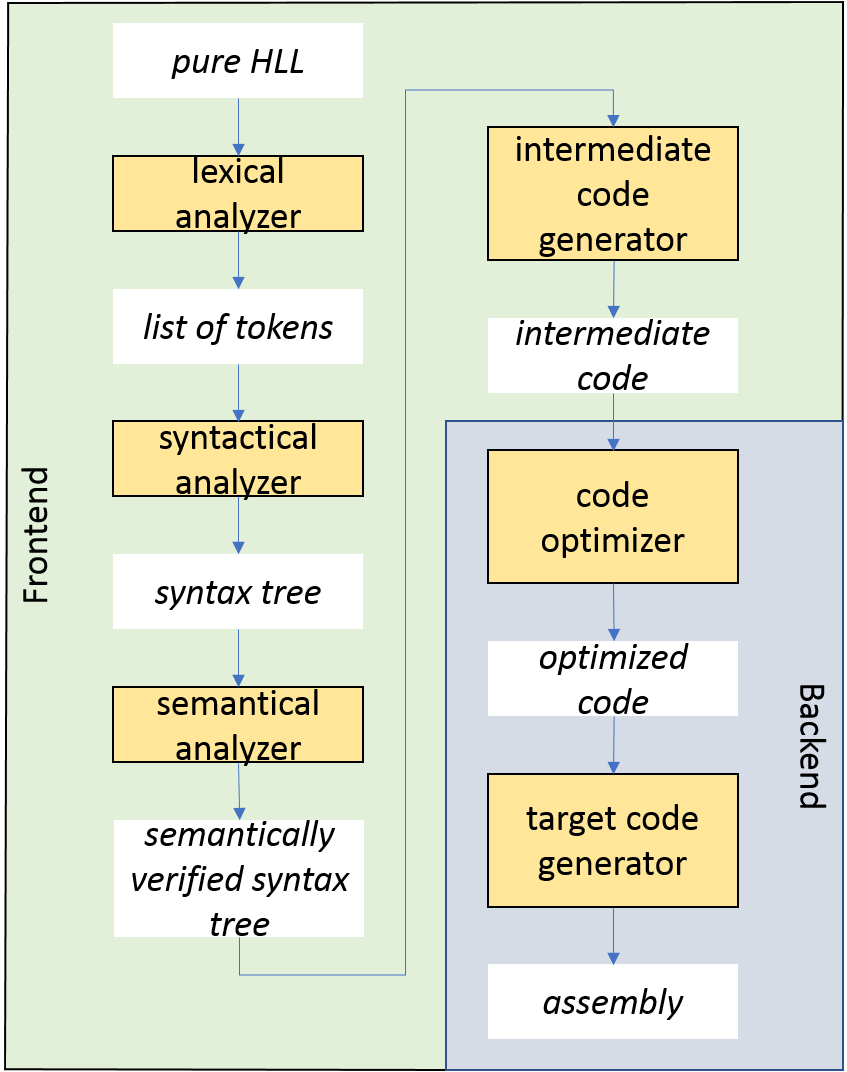
\includegraphics[width=9cm]{compiler.png}}

	\label{compiler}
	\caption{Processing chain of a compiler}
\end{figure}

x=y+1 -> id assignmentOperator id plusOperator 

Figure ~\ref{fig:compiler} shows the composition of the different components of a compiler. In a first step, a lexical analyzer, usually denoted as lexer or tokenizer, surveys the raw input sequence of characters and contracts the to be as cohesive identified words (lexemes) to a sequence of tokens in the same order. This makes it easier for the syntactical analyzer (parser) to progress because it considers the tokens as the atomic symbols instead of the initial single characters. Both lexer and parser work with some grammar based on which the symbols are bestowed semantics but while the task of a lexer is to handle a less complex regular grammar (Chomsky's level 3), which can be realized using regular expressions, parsers must cope with context-free grammars (Chomsky's level 2) and normally we would want the parser to produce a tree structure incorporating precedence. The lexer can also be used to remove unnecessary white space and comments. More about the process can be read in the next chapter.

https://stackoverflow.com/questions/2842809/lexers-vs-parsers

%If the stream of symbols does not fit the grammar, the lexer/parser should report an error.

%Lexer:
%For example: the instruction 'SKIP', which will be used to indicate
%that the program should do nothing at this point, can be expressed
%by directly matching the next four characters of the string input
%against 'SKIP'
%
%on the other hand, if you want to match a set of combinations of characters
%for a variable name for example, like usually in programming languages,
%they can start by a letter or an underscore and then any variation
%of letters, underscores and digits, it would be tedious to try every
%possibility. Therefore regular expressions are a way to specify patterns
%and most practical programming languages have an implementation to
%search a string according to these patterns.

After the syntactical analysis, there can be a semantical analysis that cross-checks the validity of the constructed syntax tree or sanitizes it, e.g. the typing in a variable assignment statement like:

\begin{equation}
	x=y+1
\end{equation}

Do variable (x) and the expression assigned to it (y+1) actually match in their respective type of data? Since the type of the variable may be fixated (declared) far off the assignment instruction, it probably won't reside in the same branch/grammar production rule path. Moreover, the namespace for variables may be shared with other entities like functions, so it might make sense to examine whether the idenfitier does in fact denote a variable. Thus the semantical analyzer exposes a verified syntax tree.

The Intermediate Code Generator translates the syntax tree into another intermediate representation, which serves as an interface between the high level language and the platform. The last two steps (Code Optimizer and Target Code Generator) can then be replaced per setup, so the other components are left untouched.

The program verifier as described in this paper is inserted right after the syntactical analyzer. It would ideally be done after a semantical analysis but the contemplated language and the samples are simple enough that such won't be required. Nowadays, the described analyses are often processed incrementally in background threads parallel to the programmer writing code and, in this way, assisted deductive program verification can be provided on-the-fly as well but it and verification in general are rather subject to specialized languages at this point in time. Examples for such languages are Spec\#, an extension to C\# or JML (Java Modeling Language), which seeks to introduce verification specifications in Java by wilily wrapping the additional semantics required in comments.

%\begin{tikzpicture}
%	\node {Lexical analyzer}
%	child { node {Syntactical analyzer} edge from parent [->] node [left] {stream of tokens} }
%		child { node {abc} }
%	};
%\end{tikzpicture}

\begin{figure}[H]
	\centering
	{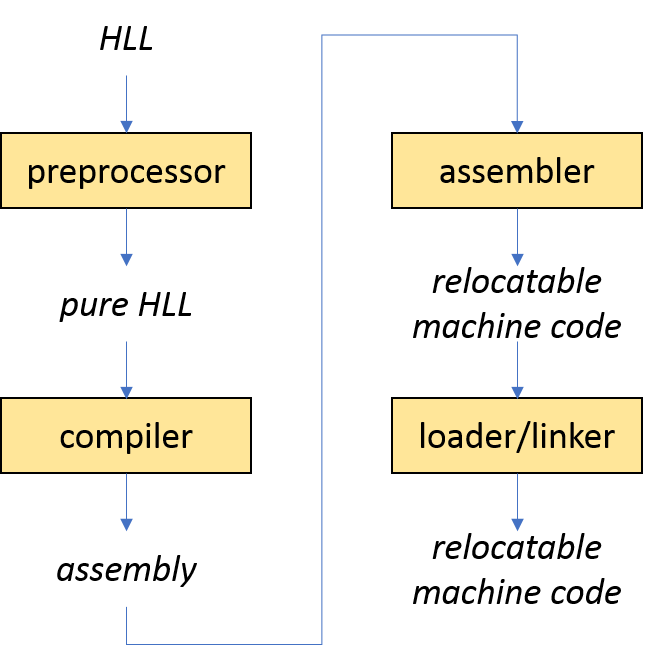
\includegraphics[width=9cm]{HLLtoMC.png}}

	\label{fig:HLLtoMC}
	\caption{High level language to machine code}
\end{figure}

%\begin{tikzpicture}
%    \node {A}
%    child { node {B} edge from parent [->] node [left] {\tiny 1} }
%    child { node {C} 
%        child { node {D}  }
%        child { node {E}  }
%        edge from parent [->] node [right] {\tiny 2}
%    }
%    ;
%\end{tikzpicture}

\section{On languages and grammars}
The considered programs are a made up from a sequence of symbols of a given alphabet. A sequence of symbols is said to be a \textit{word}.

\begin{definition}
	An alphabet is a set of symbols.
\end{definition}

\begin{definition}
	A word is a string or finite sequence of symbols (associated to a specific alphabet).
\end{definition}

\begin{figure}
	\begin{center}
	\begin{tabular}{c c}
		\{a, b, c\} & \{aaba, bbb, acb\}
	\end{tabular}
	\end{center}
\end{figure}

To later derive a meaning from it, some code must be established in advance and not just any word shall be accepted by the compiler but a well-defined set of words as denoted by a formal 'language'.

\begin{definition}
	A language is a set of words. Since those sets are most oftenly infinite, a language is commonly described by a predicate.
\end{definition}

Ex: A language may be designated by the notation of a regular expression like for instance \textit{a*b}, the asterisk being a quantifier for the preceding symbol, indicating ``an arbitrary number of'', so the given example would encompass the words \textit{b}, \textit{ab}, \textit{aab}, \textit{aaab}, \textit{aaaab} and so on.

Since languages as defined above alone still lack a proper structure to bind semantics to, the concept of grammars is to be introduced. Those consist of a set of production rules to span a language, chunk and organize their words into a tree structure, the syntax tree. Grammars always relate to a language and are formalized as following:

\begin{definition}
	A grammar is a tuple of a set of variables (also called non-terminals), terminal symbols, production rules and a starting symbol.
	\[G = (V, T, P, S)\]
	
	V - set of non-terminal symbols or variables
	T - set of terminal symbols
	P - production rules
	S - starting symbol
\end{definition}

\begin{grammar}
	<exp> ::= <exp> + <exp>
	\alt <exp> * <exp>
	\alt id

	<boolExp> ::= <boolExp> \&\& <boolExp>
	\alt <boolExp> \textbar\textbar <boolExp>
	\alt <exp> compOp <exp>
	\alt true
	\alt false
\end{grammar}

The example displays a usual notation similar to \textit{Backus-Naur Form}\footnote{\url{http://matt.might.net/articles/grammars-bnf-ebnf/}} of grammars that will also be used throughout this paper. In a mathematical representation it would be:

(V={exp, boolExp},
T={id, +, *, \&\&, \textbar\textbar, compOp, true, false},
P={
	{exp, {
		{exp, +, exp},
		{exp, *, exp},
		id
	}},

	{boolExp, {
		{boolExp, \&\&, boolExp},
		{boolExp, \textbar\textbar, boolExp},
		{exp, compOp, exp},
		true,
		false
	}}
},
S={exp})

This assumes that \textit{exp} is indeed the starting symbol, which is not quite clarified in the first notation and will instead be separately stated when needed. Variables are those that appear on the left-hand side of the production rules and form the non-terminal nodes of the syntax tree. Terminals are atomic symbols, which means they cannot be split up any further and become leaves of the syntax tree. They can only be found on the right-hand side of the rules. Furthermore, production rules tell how the input words shall be broken down into variables and terminals. The starting symbol (or set thereof) determines what rule(s) to regard on the highest level. The pipe or vertical line symbol \textit{\textbar} means an alternative. Thus the variable \textit{exp} can either be derived to \textit{exp + exp}, \textit{exp * exp} or \textit{id} here.

To explain certain traits of grammars and work towards the type that provides for the features needed later on, next some examples are to be inspected and transformed accordingly.

\subsection{Ambuigity, Associativity, Precedence}

In a first step, the grammar of ~\ref{figure:ambGrammar} shall depict the concatenation of id terminals by the + operator, namely the infix notation of addition.

\begin{figure}
	\label{ambGrammar}

	\begin{grammar}
		<exp> ::= <exp> + <exp>
		\alt id
	\end{grammar}
\end{figure}

When applying that grammar to an input \textit{id+id+id}, the two different syntax trees shown in figure ~\ref{fig:ambGrammarTree} can be derived.

\begin{figure}
	\label{ambGrammarTree}
	\caption{syntax trees of the example grammar}

	\begin{center}
	\begin{tabular}{c c}
	\Tree[
		.exp
		 [
			.exp
			 [
				.exp \textit{id}
			 ]
			 + 
			[
				.exp \textit{id}
			 ]
		 ]
		 +
		 [
			.exp \textit{id}
		 ]
	]
	&
	\Tree[
		.exp
		 [
			.exp \textit{id}
		 ]
		 +
		 [
			.exp
			 [
				.exp \textit{id}
			 ]
			 + 
			[
				.exp \textit{id}
			 ]
		 ]
	]
	\end{tabular}
	\end{center}
\end{figure}

That means the derivation process is not definite. Even with the arithmetical addition of two numbers being associative and commutative (Abelian), ambiguousness in grammars is not really desired (except if it is an operator parser handling them). There shall exist no more than one possible syntax tree for the same input and grammar. Telling if a grammar is ambiguous in general is undecidable.\footnote{\url{https://en.wikipedia.org/wiki/Ambiguous_grammar\#Recognizing_ambiguous_grammars}} However, the ambiguity at hand is induced obviously because it is unclear whether the addition operator binds left or right side. This can be taken care of by rewriting the production rules to not include the same non-terminal on both ends.

\begin{figure}
	\label{ambGrammarFixedRight}

	\begin{grammar}
		<exp> ::= id + <exp>
		\alt id
	\end{grammar}
\end{figure}

\begin{figure}
	\label{ambGrammarFixedLeft}

	\begin{grammar}
		<exp> ::= <exp> + id
		\alt id
	\end{grammar}
\end{figure}

The grammar of ~\ref{fig:ambGrammarFixedRight} has the non-terminal situated at the ending, its syntax trees grow on the right side (rightmost derivation). The grammar of ~\ref{fig:ambGrammarFixedLeft} has the non-terminal situated at the beginning, its syntax trees grow on the left side (leftmost derivation). With the addition being commutative, it does not matter semantics-wise but in order to elucidate another point about leftmost derivation, it shall be persevered. In the following step, the grammar is extended by multiplication.

\begin{figure}
	\label{ambGrammarPrec}

	\begin{grammar}
		<exp> ::= <exp> + id
		\alt <exp> * id
		\alt id
	\end{grammar}
\end{figure}

\begin{figure}
	\label{ambGrammarDiffSemantics}
	\caption{syntax trees of the example grammar with different semantics}

	\begin{center}
	\begin{tabular}{c c}
	\Tree[
		.exp
		 [
			.exp
			 [
				.exp \textit{id}
			 ]
			 + 
			[
				.exp \textit{id}
			 ]
		 ]
		 *
		 [
			.exp \textit{id}
		 ]
	]
	&
	\Tree[
		.exp
		 [
			.exp \textit{id}
		 ]
		 +
		 [
			.exp
			 [
				.exp \textit{id}
			 ]
			 * 
			[
				.exp \textit{id}
			 ]
		 ]
	]
	\end{tabular}
	\end{center}
\end{figure}

Again an example input \textit{id+id*id} yields two different syntax trees as visible in ~\ref{ambGrammarDiffSemantics}. Moreover, they entail different semantics. When evaluating the semantics of an expression like applying the mathematical operations of addition and multiplication, it is not desired to re-synthesize the string containing the mathematical expression as that would again call for the necessity of analyzing the structure but rather to directly work on the syntax tree step by step. The children of a node would recursively be conflated before advancing to the parent. So in figure ~\ref{fig:ambGrammarDiffSemantics}, the left tree would execute the addition first and the result becomes a factor in the multiplication, which amounts to a different value than what the mathematical expression \textit{id+id*id} denotes. The multiplication must be carried out before the sum. This raises the question on how to enforce operator precedence within a grammar. The operation of higher precedence has to be on a deeper tree level. The solution is to split the grammar into more stages of variables.

\begin{figure}
	\label{ambGrammarPrecFixed}

	\begin{grammar}
		<exp> ::= <exp> + <mult> | <mult>
		<mult> ::= <mult> * id | id
		\alt id
	\end{grammar}
\end{figure}

Now, in the grammar of ~\ref{fig:ambGrammarPrecFixed}, the + and the * operators are disconnected. Only the <mult> variable is able to contain multiplication and it cannot go back to <exp>. The purpose of <exp> is to realize summation but it can derive to occurences of <mult>. So it is a one-way street and the sum derivation happens at the upper levels. The ambiguity was eliminated as well. The raison d'être of the second rule of <exp> is for the case that there is no summation involved, it should go straight to <mult> then. The second rule of <mult> functions as a terminator, else the tree would keep on growing and maybe there is no multiplication at all.

\textit{id+id+id*id*id+id}

\begin{figure}
	\label{ambGrammarPrecFixedTree}
	\caption{syntax trees of the example grammar with different semantics}

	\begin{center}
	\begin{tabular}{c}
	\Tree[
		.exp
		 [
			.exp
			 [
				.exp
				 [
				 	.mult \textit{id}
				  ] 
			  ]
			 + 
			[
				.mult
				 [
					.mult
					[
						.mult \textit{id}
					]
					*
					[
						\textit{id}
					]
				 ]
				*
				[
					\textit{id}
				]
			 ]
		  ]
		 +
		 [
			.mult \textit{id}
		  ]
	]
	\end{tabular}
	\end{center}
\end{figure}

In summarization, to fix associativity, the recursivity of the rules has to be adjusted. To fix precedence, a hierarchy of non-terminals has to be established. This information will later be adduced when designing the language whose words shall be verified and that is going to be implemented.

\subsection{The problem with left recursion}

When writing a grammar, it should be considered that a parser will have to be able to work with it. In a grammar as depicted in ~\ref{grammarLR} with the starting symbol being <exp>, a top-down parser has to make a decision whether to pick the rule <exp> ::= <exp> + id or <exp> ::= id. The basis for a specific decision is the input string. When entering the <exp> variable, the type of parser that will be illustrated here would investigate the first part of the first production rule, which again is <exp>. Without having made any progress, it finds itself the same situation, the parser will try to derive <exp> and see <exp> as the way to go. It turns out to be an infinite loop. This is why left recursion should be avoided.

\begin{figure}
	\label{grammarLR}

	\begin{grammar}
		<exp> ::= <exp> + id
		\alt id
	\end{grammar}
\end{figure}

Exp()
{
	Exp()
	id
}

Exp()
{
	id
	Exp()
}

To retain the generated language yet still get rid of left recursion, there is a simple conversion prescript.

\begin{figure}
	\label{ambGrammarPrecFixedTree}
	\caption{elimination of left recursion}
	
	\begin{center}
		\begin{tabular}{p{5cm} p{5cm}}
			\begin{grammar}
				<A> ::= <A> \textcolor{red}{\textit{abc}}
				\alt \textcolor{blue}{def}
			\end{grammar}
			%\\
			\begin{grammar}
				<A> ::= \textcolor{blue}{\beta} <A'>
				<A'> ::= \textcolor{red}{\alpha} <A'>
				\alt \epsilon
			\end{grammar}
		\end{tabular}
	\end{center}
\end{figure}

\begin{figure}
	\label{ambGrammarPrecFixedTree}
	\caption{elimination of left recursion}

	\begin{center}
		\begin{tabular}{p{5cm} p{5cm}}
			\begin{grammar}
				<A> ::= <A> \textcolor{red}{\alpha}
				\alt \textcolor{blue}{\beta}
			\end{grammar}
			\\
			\begin{grammar}
				<A> ::= \textcolor{blue}{\beta} <A'>
				<A'> ::= \textcolor{red}{\alpha} <A'>
				\alt \epsilon
			\end{grammar}
		\end{tabular}
	\end{center}
\end{figure}

Another non-terminal is inserted that may right-recursively spawn new instances of \alpha or end with \epsilon which is the empty word. \epsilon does not take any token from the input. Now, \alpha and \beta may be substituted by any sequence of variables/terminals. To reform the above example with <exp> and match the conversion pattern, \alpha corresponds to + <mult> and \beta corresponds to <mult>. It is shown in ~\ref{fig:grammarExpRR}.

\begin{figure}
	\label{grammarExpRR}
	\caption{exp with right recursion}

	\begin{center}
		\begin{tabular}{c c}
			\begin{grammar}
				<exp> ::= <exp> \textcolor{red}{+ <mult>}
				\alt \textcolor{blue}{beta}
			\end{grammar}
			\\
			\begin{grammar}
				<exp> ::= \textcolor{blue}{<mult>} <exp'>
				<exp'> ::= \textcolor{red}{+ <mult>} <exp'>
				\alt \epsilon
			\end{grammar}
		\end{tabular}
	\end{center}
\end{figure}

On top of that, the pattern can be extended like in ~\ref{fig:grammarElimLRMultiple}.

\begin{figure}
	\label{grammarElimLRMultiple}
	\caption{elimination of left recursion with multiple instances of \alpha and \beta}

	\begin{center}
		\begin{tabular}{c c}
			\begin{grammar}
				<A> ::= <A> \textcolor{red}{\alpha_1}
				\alt <A> \textcolor{red}{\alpha_2}
				\alt <A> \textcolor{red}{\alpha_3}
				...
				\alt \textcolor{blue}{\beta_1}
				\alt \textcolor{blue}{\beta_2}
				\alt \textcolor{blue}{\beta_3}
				...
			\end{grammar}
			\\
			\begin{grammar}
				<A> ::= \textcolor{blue}{\beta_1} <A'>
				\alt \textcolor{blue}{\beta_2} <A'>
				\alt \textcolor{blue}{\beta_3} <A'>
				...
				<A'> ::= \textcolor{red}{\alpha_1} <A'>
				\alt \textcolor{red}{\alpha_2} <A'>
				\alt \textcolor{red}{\alpha_3} <A'>
				...
				\alt \epsilon
			\end{grammar}
		\end{tabular}
	\end{center}
\end{figure}

Lastly, in order to produce a LL(1) grammar, non-determinism shall be erased. That means that the parser must be able to deduce which rule to use by only looking at the next token of the input string and not tracing back. Common prefixes in the production rules of a variable have to be excluded to realize that feature. That process is also called left factoring and is visualized in ~\ref{fig:grammarExpLeftFactoring}.

\begin{figure}
	\label{grammarExpRR}
	\caption{exp with right recursion}

	\begin{center}
		\begin{tabular}{c c}
			\begin{grammar}
				<A> ::= \alpha \beta_1
				\alt \alpha \beta_2
				...
			\end{grammar}
			\\
			\begin{grammar}
				<A> ::= \alpha <A'>
				<A'> ::= \beta_1
				\alt beta_2
				...
			\end{grammar}
		\end{tabular}
	\end{center}
\end{figure}

LL(1) stands for processing the input from left to right and having a lookahead of only 1 token, so no back tracing required. Using a parsing table, a LL(1)-parser can directly make the rule picking decision by knowing the current non-terminal and the next terminal obtained from the input sequence. Before moving on to the actual language going to be used, the process of constructing a LL(1) parser table shall be outlined.

First
First is applied on a production rule
To obtain the set of Firsts of a variable, all of its production rules are introspected. For each rule, if the first symbol is a terminal that terminal is added to the set and the rule has finished. If it is a non-terminal, the First procedure is recursively invoked on the non-terminal and its resulting terminals relayed to the parent. Should the terminal be the empty word, since this leaves the input stream untouched, instead of adding \epsilon to the set, First will be applied to the next symbol of the parent.

Follow
To get the Follow terminals of a variable, all of the grammar's production rules are checked for occurences of the variable. If the occurence is the last symbol of the production rule, the Follow of the variable whose production rule it is will be used instead. Otherwise, the First of the remainder of the production rule will be used.

Now there are different classes of grammars. Depending on it, the required strategy of a parser will look different. The later introduced language will suffice LL(1). This is why the following steps explain the constraints and the construction of a LL(1) grammar.

How to enforce unilateral associativity?

This can be done by having no production rule 

How to enforce operator precedence?

Both the tokenizer and parser rely on the same grammar in the sense that the tokenizer produces the same-named terminal instances for the parser.

There are certain requirements a grammar should fulfill in order to make the semantics precise and proper. First off, it should be unambiguous, the input string must not be interpretable in more than one way but yield exactly one syntax tree. This is achieved by fixing the associativity.

E->E+E

E->E+id/id

left associative, tree can grow on left side

E->id+E/id

right associative, tree can grow on right side

Moreover, a certain precedence of operators is desired, like the application of a multiplication should come before addition.

E->E+T/T
T->T*F/F

split it in levels 

recursion left-recursion or right-recursion, left-recursion should be avoided

A()
{
	A()
	a
}

infinite loop (in top-down parsers) since no tokens are removed from the stream, same situation

grammar generated certain language

same language can be constructed with right-recursion grammar by transformation

A->Aa/b

A->bA'
A'->aA'/eps

deterministic grammar: no backtracking (production rule can be determined safely by only looking at next token), no common prefixes (common prefixes problem), left factoring

A->ab/ac/ad

A->aA'
a'->b/c/d

shifts decision making process by inserting intermediate stops
This creates more non-terminals and increases the tree depth but spans a LL(1) grammar that can predict the right production rule to use by looking at only the next token. It can therefore be solved with a simple lookup table. NxT->P

http://pages.cs.wisc.edu/~fischer/cs536.s15/lectures/L9.4up.pdf

\textemdash{}

\Tree[.E [.E [.E \textit{id} ] * [.E \textit{id} ] ] + [.E \textit{id} ] ]

\textemdash{}

The different parsers 

Construction of the grammar

%errorhandler+symbol table manager for all modules

grammar (context-free) LR1

Hoare needs to go from right to left, parser from left to right >
cannot be parallel

left most derivation (replace left most variable), right most derivation
(exp example)

ambiguous grammars (more than one tree for same string), make them
unambiguous, left/right associativity, operator precedence

modify grammar, for left associativity -> left recursive -> E>E+id|id,
precedence -> different levels -> E>E+T|T T>T{*}F|F

with fixed associativity, it becomes unambiguous

left recursion would cause infinite loop A\{ A(); a)

top-down-parser have problems with LR, A>ba{*} -> A>bA' A'>eps|aA'
<=> A>aA/B, LR to RR conversion

deterministic, non-deterministic grammar -> different options for
productions -> back-tracking, common prefixes problem, left factoring
A>ab|ac|ad -> A>aA' A'>b|c|d

\paragraph{}

%\newenvironment{grammar}[2]{\begin{verbatim}}{\end{verbatim}}

\begin{grammar}
	<id> ::= [a-zA-Z] [a-zA-Z0-9\_]*

	<num> ::= [1-9] [0-9]*
	\alt '0'
\end{grammar}

Using First and Follow, the predictive parser table for the LL(1) grammar can be spanned.

\begin{table}
	\begin{tabular}{c|c|c|c|c|c|c}
		\backslashbox{non-terminal}{terminal} &
		id + * \( \) \$ \\
		\hline
		exp & exp->term erest & & \\
		\hline
	\end{tabular}
\end{table}

\section{Core language}

\section{Semantics}

The semantics are inductively defined, which means to make sense of a construct, its components are recursively examined.

expression:
To obtain the semantics of an expression, the involved variables need to be resolved for their current value.

condition:


\chapter{How to prove}

\section{From operational semantics}
assertions, extension of language
partial correctness, total correctness

The idea now is to use the semantics defined at the end of the previous chapter in order to make statements about the execution of a given program. This is similar to actually running the program, subsequentially traversing the entered lines of code and keeping memory of the current variable values. The mapping of all variables used inside the program as well as additional helper variables to specific values is called a state. As according to the introduced language, only the assignment instruction has the ability to alter the state.

%var(prog) - set of variables occuring in the program
%value(var \in var(prog)) - domain of the values the variable can be applied to (as specified by the data type)
%states(prog) - set of all states

\section{Transition to Hoare calculus}
%\begin{align}
%\begin{split}
SKIP AXIOM:
	\begin{equation}
		\{p\}\ SKIP\ \{p\}
	\end{equation}
//
ASSIGNMENT AXIOM:
	\begin{equation}
		\{p[u:=t]\}\ u:=t\ \{p\}
	\end{equation}
//
COMPOSITION RULE:
	\begin{equation}
		\dfrac{\{p\}S_1\{r\},\{r\}S_2\{q\}}{\{p\}\ S_1;S_2\ \{q\}}
	\end{equation}
//
CONDITIONAL RULE:
	\begin{equation}
		\dfrac{\{p\wedge B\} S \{p\}}{\{p\} IF\ B\ THEN\ S_1\ ELSE\ S_2\ FI\{q\}}
	\end{equation}
//
LOOP RULE:
	\begin{equation}
		\dfrac{\{p \wedge B\}S\{p\}}{\{p\}\ WHILE\ B\ DO\ S\ OD\ \{p \wedge \neg B\}}
	\end{equation}
//
CONSEQUENCE RULE:
	\begin{equation}
		\dfrac{p \to p_1,{p_1}S{q_1},q1 \to q}{{p}\ S\ {q}}
	\end{equation}
%\end{split}
%\end{align}

The Hoare calculus is a proof system consisting of axioms and rules that establish a relationship between pre- and postconditions of a set of basic programming constructs. Each of them is embodied by a Hoare triple {p} S {q}, p denoting the precondition, S the program section and q the postcondition. The horizontal bar is a fancier notation an implication: If all of the conditions above the bar are correct, the statenents below are true as well.

The SKIP axiom states that it does not cause any change, which makes sense, as the instruction does infact nothing.

In the assignment axiom, it is indicated that the precondition can be derived from the postcondition by replacement of each of the occurences of the variable by the assigned expression. Example:

%\DeclarePairedDelimiter\Hoare{\,\llparenthesis\,}{\,\rrparenthesis\,}
%\begin{document}
%\[
%    \Hoare{x > 0} P \Hoare{y \cdot y < x}
%\]

\newenvironment{hoare}[0]{\begin{equation}}{\end{equation}}

\begin{hoare}
	\{x=10[x:=2*x]\} x=2*x \{x=10\} \equiv \{2*x=10\} x=2*x \{x=10\}
\end{hoare}

Resolving that precondition formula for x yields 5. So in order to arrive at a state z with z(x)=10 after the program section \textit{x=2*x}, x must have hold the value 5 just previously.

The composition rule displays a transitive property. A sequential composition of two program parts can be evaluated by taking a look at one part and passing an obtained postcondition to the second part as its precondition, respectively vice versa when verifying from right to left.

Encountering a selection is somewhat more troublesome. Either the B condition is found true at the point of execution whereupon S\_1 must be processed or B is evaluated to false and the processor pursues S\_2. Therefore, it is one of those two cases and the triple tries to account for both.

The rule for while loops is particularly sophisticated. It requires one to think of a condition that holds true before and after each iteration, which is why such a condition is called a loop invariant p. After the loop has finished, p must still be true and the loop condition B untrue. Searching for p is a non-trivial, undecidable venture and a research matter up for discussion in the \textit{Challenges} section.

Finally, the consequence rule serves as an interface and makes an important point: A precondition can always be substituted by one that encompasses a previous one, i.e. is a stronger assertion. Similarly, a postcondition may be weakened anytime.

Some more notes about the use of the calculus and the effects of the constructs:
As the system depicts only the mapping of relations, the order of evaluation is not quite fixed. The analysis of a program may commence from the beginning onwards or push up from the ending, or even a combination thereof. However, there are a couple of reasons why the second option seems preferable.

The assignment axiom presents an explicit instruction to get the precondition from the postcondition. Going from left to right requires more thinking and case distinction.

Assuming that the precondition p does not include the modified variable x, it would be intuitive that the strongest postcondition just adds the clause of x possessing the newly assigned value:
\begin{hoare}
\{p\} x=2 \{p\wedge x=2\}
\end{hoare}

If p does not contain x and the assigned value is a function of x, as there is no presumption about x, p will stay the same:
\begin{hoare}
\{p\} x=x+2 \{p\}
\end{hoare}

If p contains x and the value expression does not, the clauses in p that contain x would have to be discarded and and x possessing the newly assigned value added:
\begin{hoare}
\{p\} x=2 \{p[x:=]\wedge x=2\}
\end{hoare}

\section{Challenges}
\subsection{Finding invariants}

A main challenge of using the Hoare calculus consists of finding fitting loop invariants. Those invariants are supposed to imply the postcondition.

p -> 

\subsection{Resolving implications}

\section{Outlook on parallelism}
In parallel programs, there is more than one program flow running concurrently. This allows for greater flexibility, modularization and can also boost the performance by scattering the workload on different processors. On the other side, these enhancements call for additional management handling because, at some point, the routines are still to collaborate in order to realize an integral system and besides that should not interfere with one another. A distinction is made between parallel programs that access a common memory like shared variables to exchange information and a distributed system where the components communicate passing explicit messages.

With the new set of possibilities and mingling cases it becomes much harder to verify such systems.

When dealing with parallelism, the components need to be coordinated
to not interfere each other or trigger a deadlock. Verify absence
of errors. Discipline of program verifications commits itself to systematically
approaching the proof of accuracy, that is, checking a model against
a specification.

sequential programs are the basis, they only possess one flow of control

of course those characteristics are also desired for parallel programs,
additionally:

no interference
no deadlocks
maybe correct without fairness or enforcement of a certain fairness

//parallel/distributed
interference free
deadlock free/livelock
fairness

\chapter{Implementation}

\section{Java}
Java/JavaFX/MVC

\section{Lexer, parser}

save position of tokens -> syntax errors

\section{Hoare}

\section{Exception handling}

\section{GUI}

\subsection{Editor}
\subsection{Display of tokens/syntax tree}
\subsection{Syntax chart with Hoare decoration}

\chapter{Excursions}
\section{Shape analysis}
\section{Model checking}
automata, petri nets
\section{Alternative logics}
linear temporal logic (LTL), timed computation tree logic (TCTL)

\chapter{Fazit}
\section{Summerization}
\section{Remaining problems}
what is not covered, parallelism, deadlock, inference, fairness
\section{Extendabilities}

\chapter{References}

modern languages no null objects, frequent source of error (NullPointerException)
ProofCarryingCode, code devoid of proofs

correctness important, program has to fulfill specifications/properties

correct results
termination
no runtime errors

operational reasoning usual in programmer's everyday life but bad
denotational reasoning
fixed point semantics

here: axiomatic reasoning, predicate logic to specify properties
assertions

axiomatic approach limits:
verification, not development
only input/output characteristics, not of finite/infinite operations
no fairness assumptions

%temporal logic:
%liveness properties
%fairness

classes of programs
while program
%fine-tuned verification methods for each class

theory of computability general verification undecidable, finite-state systems -> possible
model checking -> program is model of specification?
program analysis -> similar to model checking, dynamic behavior analyzed, has variable value at control point?

%deductive verification automates axiomatic approach
%ApplicativeCommonLisp
%Isabelle/HOL



usual desired features of sequential programs:

partial correctness: if the algorithm returns a result (terminates),
it is correct in reference to the statement of the problem. The termination
is not guaranteed.

termination: the algorithm terminates for all designated inputs, else
the algorithm is said to diverge

no run time errors: no undefined operations like division by zero
occur

example: different sorting algorithms

mathematical logic

what is correctness

the disadvantages of the axiomatic approach are that those rules are
only suited for the verification, not for the development of a program,
only the behavior in reference to input/output, not considering finite/infinite
executions (operating system), fairness is ignored

proof system for each class of programs

\textemdash{}

\textemdash{}

\newpage{}

\chapter*{Appendices}

Gate Lectures by Ravindrababu Ravula

% Dieser Code ist noetig, da sonst die falsche Seitenzahl im Inhaltsverzeichnis angezeigt wird
\clearpage
\phantomsection
% Die folgende Zeile sorgt dafuer, dass der Glossar im Inhaltsverzeichnis angezeigt wird.
%\addcontentsline{toc}{chapter}{Glossar}

%\nomenclature{APT}{Advanced Packaging Tool (kurz. APT) ist ein Paketverwaltungssystem das z.B. bei Debian und Ubuntu eingesetzt wird. Das Paketverwaltungssystem stellt einen Gro�teil der f�r das Betriebssystem verf�gbaren Programme und Erweiterungen bereit. Diese k�nnen durch den Benutzer meist in der Befehlszeile oder �ber eine grafische Oberfl�che installiert und konfiguriert werden. }\nomenclature{API}{Application Programming Interface (kurz API) ist eine Programmierschnittstelle die eine Anbindung von Au�en an ein bestehendes System bietet. Die Schnittstelle wird vom Hersteller der Software zur Verf�gung gestellt um Dritten die M�glichkeit eines Addons oder einer Erweiterung zu geben. Die Schnittstelle definiert dabei ein Standardformat und Standardbefehle.}
%
%\settowidth{\nomlabelwidth}{LAN}
%\printnomenclature{}

% Dieser Code ist noetig, da sonst die falsche Seitenzahl im Inhaltsverzeichnis angezeigt wird
\clearpage
\phantomsection

\bibliographystyle{plain}
\nocite{*}
\bibliography{lib}

\begin{flushleft}
\newpage{}
\par\end{flushleft}

%\include{vow}

\vspace{17.1mm}


%\section*{{\huge{}Master's thesis statement of originality}}
\section*{{\huge{}Author´s declaration}}

%\begin{verbatim}
I hereby confirm that I have written the accompanying thesis by myself, without contributions from any sources other than those cited in the text and acknowledgements.
This applies also to all graphics, drawings, maps and images included in the thesis.
%\end{verbatim}

\vspace{2cm}

\begin{center}
	\begin{tabular}{@{}p{5cm}@{}p{2cm}@{}p{5cm}}%{15cm}{@{\extracolsep{\fill}}cl}
%		\hline
		Merseburg, \today & &  \\
%		\hline
		\dotfill & & \dotfill \\
%		\hline
		\emph{Place and date} & & \emph{Signature} \\
%		\hline
	\end{tabular}
	\par
\end{center}

\newpage

\section*{{\huge{}Dedication and acknowledgements}}

%\begin{figure}[h]
%\begin{lstlisting}[backgroundcolor={\color{lightgray}},basicstyle={\normalsize\sffamily},breaklines=true,frame={leftline,bottomline,rightline,topline},language=C,numbers=left,showstringspaces=false,xleftmargin=15pt]
%#include <stdio.h> 
%main() 
%	{
%        int i;
%        for (i = 0; i<=2; i++)
%        {
%        fork();
%        setvbuf(stdout, NULL, _IOLBF, 0); //(Stream, Pufferangabe, Puffertyp, Puffergroesse)
%        printf("PID=%6d, i=%d\n", getpid(), i);
%        }
%} 
%\end{lstlisting}
%
%\caption{Modifiziertes Programm mit setvbuf()}
%\end{figure}

%\index{}$x+y=z^{2}$
\end{document}